\section{Agile Methodologies}

In the last years the Agile software development got popular due to his
different and modern way to see software as an incremental process. It
helps development teams to define what to do step by step, revolutionizing
the traditional approach that instead use to follow a sequential process.

In the Scrum method of Agile software development work is defined during
intervals called Sprints; a Sprint used to be 30 days long, but usually
teams prefer shorter sprints of two weeks.

A Sprint starts with a Sprint planning meeting: during this meeting the team
analyses the backlog and decides which tasks have highest priority in the
development process. Those tasks are then assigned to the members of the team
that reports his progress and problems during the daily Scrum meeting. At the
end of the Sprint there is a Sprint review meeting in which the team shows the
work done and analyses how to improve the next Sprint.

Using this regular cadences of work it is easy to understand how planning
software development is way easier with an Agile approach. Also reacting to
unforeseen events or changing requirements is easier than with the waterfall
approach. For this reason Agile development is also called "iterative" or
"incremental".

In the following sections we will analyse a set of techniques which are used in
Agile development to increase the productivity of the team.

\subsection{Continuous integration}

Continuous Integration is the practise, in software engineering, to merge
the developers work into the main project as soon as the task assigned is
completed. The aim of this approach is to prevent possible integration
problems: doing small changes often makes easy to track down problems and
avoids error when merging to the mainline.

This method is used most of the time in combination with automated unit tests:
after modifying the code the developer runs the unit tests to check that his
change has not compromised somebody else functionality. It is fundamental to
write tests for every new function in order to cover all the use cases and
detect anomalies before deployment.

Later were also introduced build servers to run unit tests after every commit
or merge request; in some cases build servers can also run static code analysis
and style checkers.

\subsection{Continuous delivery}

Continuous Delivery is an extension of Continuous Integration that adds regular
merges to the mainline as a part of the process. This does not mean that the
software is deployed after every commit, but it means that every change is
proved to be deployable at any time.

In particular this consists in deploying the software in a production-like
environment and run functional tests as a part of the process. Since every
change is delivered to a staging environment using an automated process we are
sure that the application can also be deployed to production at any time.

\subsection{Continuous deployment}

Continuous Deployment is the step after Continuous Delivery, it means that
every change that is committed, after running unit and functional tests, is
automatically deployed to production. This approach is obviously not feasible
in certain circumstances, for example in business cases where a feature must
wait to go live.

\begin{figure}[H]
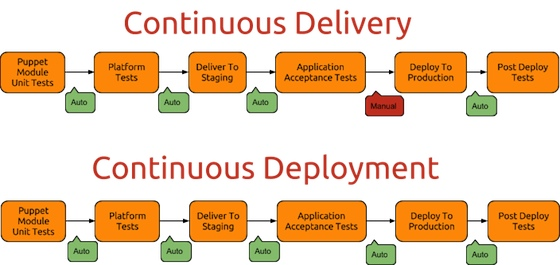
\includegraphics[width=\textwidth,height=\textheight,keepaspectratio]{Introduction/Continuous_Delivery_Continuous_Deployment.jpg}
\end{figure}
